\documentclass[sigconf]{acmart}
\usepackage{amsmath}
\usepackage{graphicx}
\usepackage{float}
\usepackage{subfig}
\usepackage{adjustbox}
\usepackage{booktabs}

\usepackage{tcolorbox} % for graphics placeholders
\newcommand{\graphicsplaceholder}[2]{%
	\begin{tcolorbox}[valign=center,width=#1,height=#2,arc=0.5mm,auto outer arc]%
		\centering%
		\sf missing graphic%
	\end{tcolorbox}%
}

\newcommand{\mytool}{Modified K Core Decomposition}
%\usepackage{lipsum}

%%
%% \BibTeX command to typeset BibTeX logo in the docs
\AtBeginDocument{%
  \providecommand\BibTeX{{%
    \normalfont B\kern-0.5em{\scshape i\kern-0.25em b}\kern-0.8em\TeX}}}

%% Rights management information.  This information is sent to you
%% when you complete the rights form.  These commands have SAMPLE
%% values in them; it is your responsibility as an author to replace
%% the commands and values with those provided to you when you
%% complete the rights form.
\setcopyright{acmcopyright}
\copyrightyear{2018}
\acmYear{2018}
\acmDOI{10.1145/1122445.1122456}

%% These commands are for a PROCEEDINGS abstract or paper.
\acmConference[Woodstock '18]{Woodstock '18: ACM Symposium on Neural
  Gaze Detection}{June 03--05, 2018}{Woodstock, NY}
\acmBooktitle{Woodstock '18: ACM Symposium on Neural Gaze Detection,
  June 03--05, 2018, Woodstock, NY}
\acmPrice{15.00}
\acmISBN{978-1-4503-XXXX-X/18/06}


%%
%% Submission ID.
%% Use this when submitting an article to a sponsored event. You'll
%% receive a unique submission ID from the organizers
%% of the event, and this ID should be used as the parameter to this command.
%%\acmSubmissionID{123-A56-BU3}

%%
%% The majority of ACM publications use numbered citations and
%% references.  The command \citestyle{authoryear} switches to the
%% "author year" style.
%%
%% If you are preparing content for an event
%% sponsored by ACM SIGGRAPH, you must use the "author year" style of
%% citations and references.
%% Uncommenting
%% the next command will enable that style.
%%\citestyle{acmauthoryear}

%%
%% end of the preamble, start of the body of the document source.
\begin{document}

%%
%% The "title" command has an optional parameter,
%% allowing the author to define a "short title" to be used in page headers.
\title{Identification of Most Influential Spreaders in Twitter Social Network using Modified K Core Decomposition in Distributed Environment}
\begin{comment}
%%
%% The "author" command and its associated commands are used to define
%% the authors and their affiliations.
%% Of note is the shared affiliation of the first two authors, and the
%% "authornote" and "authornotemark" commands
%% used to denote shared contribution to the research.
\author{TM Tariq Adnan}
%\authornote{Both authors contributed equally to this research.}
%\email{tmadnan10@gmail.com}
%\orcid{1234-5678-9012}
%\author{G.K.M. Tobin}
%\authornotemark[1]
%\email{webmaster@marysville-ohio.com}
%\affiliation{%
%  \institution{Institute for Clarity in %Documentation}
%  \streetaddress{P.O. Box 1212}
%  \city{Dublin}
%  \state{Ohio}
%  \postcode{43017-6221}
%}



\author{Md Saiful Islam}
%\email{saiful.11722@gmail.com}
\author{Tarikul Islam Papon}
\author{Shourav Nath}
\author{Touhidul Islam}
\author{Muhammad Abdullah Adnan}
\affiliation{%
  \institution{Bangladesh University of Engineering and Technology (BUET)}
  %\streetaddress{1 Th{\o}rv{\"a}ld Circle}
  \city{Dhaka}
  \country{Bangladesh}}



\affiliation{%
  \institution{Inria Paris-Rocquencourt}
  \city{Rocquencourt}
  \country{France}
}

\author{Aparna Patel}
\affiliation{%
 \institution{Rajiv Gandhi University}
 \streetaddress{Rono-Hills}
 \city{Doimukh}
 \state{Arunachal Pradesh}
 \country{India}}

\author{Huifen Chan}
\affiliation{%
  \institution{Tsinghua University}
  \streetaddress{30 Shuangqing Rd}
  \city{Haidian Qu}
  \state{Beijing Shi}
  \country{China}}

\author{Charles Palmer}
\affiliation{%
  \institution{Palmer Research Laboratories}
  \streetaddress{8600 Datapoint Drive}
  \city{San Antonio}
  \state{Texas}
  \postcode{78229}}
\email{cpalmer@prl.com}

\author{John Smith}
\affiliation{\institution{The Th{\o}rv{\"a}ld Group}}
\email{jsmith@affiliation.org}

\author{Julius P. Kumquat}
\affiliation{\institution{The Kumquat Consortium}}
\email{jpkumquat@consortium.net}

%%
%% By default, the full list of authors will be used in the page
%% headers. Often, this list is too long, and will overlap
%% other information printed in the page headers. This command allows
%% the author to define a more concise list
%% of authors' names for this purpose.
\renewcommand{\shortauthors}{Trovato and Tobin, et al.}

\end{comment}
%%
%% The abstract is a short summary of the work to be presented in the
%% article.
\begin{abstract}
  A clear and well-documented \LaTeX\ document is presented as an
  article formatted for publication by ACM in a conference proceedings
  or journal publication. Based on the ``acmart'' document class, this
  article presents and explains many of the common variations, as well
  as many of the formatting elements an author may use in the
  preparation of the documentation of their work.
\end{abstract}

%%
%% The code below is generated by the tool at http://dl.acm.org/ccs.cfm.
%% Please copy and paste the code instead of the example below.
%%
\begin{CCSXML}
<ccs2012>
 <concept>
  <concept_id>10010520.10010553.10010562</concept_id>
  <concept_desc>Computer systems organization~Embedded systems</concept_desc>
  <concept_significance>500</concept_significance>
 </concept>
 <concept>
  <concept_id>10010520.10010575.10010755</concept_id>
  <concept_desc>Computer systems organization~Redundancy</concept_desc>
  <concept_significance>300</concept_significance>
 </concept>
 <concept>
  <concept_id>10010520.10010553.10010554</concept_id>
  <concept_desc>Computer systems organization~Robotics</concept_desc>
  <concept_significance>100</concept_significance>
 </concept>
 <concept>
  <concept_id>10003033.10003083.10003095</concept_id>
  <concept_desc>Networks~Network reliability</concept_desc>
  <concept_significance>100</concept_significance>
 </concept>
</ccs2012>
\end{CCSXML}

\ccsdesc[500]{Computer systems organization~Embedded systems}
\ccsdesc[300]{Computer systems organization~Redundancy}
\ccsdesc{Computer systems organization~Robotics}
\ccsdesc[100]{Networks~Network reliability}

%%
%% Keywords. The author(s) should pick words that accurately describe
%% the work being presented. Separate the keywords with commas.
\keywords{datasets, neural networks, gaze detection, text tagging}

%% A "teaser" image appears between the author and affiliation
%% information and the body of the document, and typically spans the
%% page.
%%
%% This command processes the author and affiliation and title
%% information and builds the first part of the formatted document.
\maketitle

\section{Introduction}
Social Networks have gained remarkable popularity in the past few decades. A huge
number of people are using social networking sites like Facebook, Twitter, Google+, LinkedIn etc. The heavy reliance on social networking sites causes them to generate massive data. Online social networks play a major role in the diffusion of information~\cite{bakshy2012role}. Since social network has great influence on society, the recent focus is on extracting valuable information from this huge amount of data. Events, issues, interests etc. happen and evolve very quickly in social networks and their capture, understanding, visualization, and prediction are becoming critical expectations from both end-users and researchers. Therefore researchers in recent years have developed a variety of techniques and models to capture information diffusion in online social networks, analyze it, extract knowledge from it and predict it~\cite{agichtein2008finding,doerr2012rumors}. 

Micro-blogging is an emerging form of communication. One of the most notable micro-blogging services is \emph{Twitter}. It allows \emph{twitterers} to publish tweets (with a limit of 140 characters). \emph{Twitter} employs a social-networking model called ``following'', in which each \emph{twitterer} is allowed to choose who she wants to follow without seeking any permission. Conversely, she may also be followed by others without granting permission first. In one instance of ``following'' relationship, the \emph{twitterer} whose updates are being followed is called the ``friend'', while the one who is following is called the ``follower''. \emph{Twitter} has gained huge popularity since the first day that it was launched~\cite{milstein2008twitter}. It has also drawn increasing interests from research community~\cite{cheng2009inside}. Many analysis have been done on the dataset of twitter including identification of the most influential spreader~\cite{pal2011identifying,weng2010twitterrank}. We discuss the state-of-art in details in the next section. 

Information diffusion is a vast research domain and has attracted research interests from many fields, such as physics, biology, etc. The diffusion of innovation over a network is one of the original reasons for studying networks and the spread of disease among a population has been studied for centuries~\cite{anderson1992infectious,heesterbeek2000mathematical,keeling2008modeling}. The knowledge of the spreading pathways through the network of social interactions is crucial for developing efficient methods to either hinder spreading in the case of diseases, or accelerate diffusing in the case of information dissemination. The information diffusion model is based on three fundamental questions: \emph{(i) Which pieces of information diffuse the most, (ii) How, why and through which paths information is diffusing, and will be diffused in the future, (iii) Which members of the network play important roles in the spreading process?}

In this paper we are mainly focusing on the third question. Identifying the most influential spreaders in a network is critical for ensuring efficient diffusion of information, which allows to control the outbreak of any kind of epidemic \cite{pastor2002immunization,PhysRevLett.91.247901}, utilize the limited resources to optimize the information propagation [20], successful e-commercial advertisements \cite{Leskovec:2007:DVM:1232722.1232727,lu2012recommender}, optimize the use of limited resources to facilitate information propagation \cite{chen2013information} etc. In large social network graph the nodes having the largest degree are often considered as the most influential spreader~\cite{pastor2001epidemic}. However, recent studies have shown that the most connected people are not the most influential spreader. Kitsak et al.~\cite{kitsak2010identification} showed that the best spreaders are not necessarily the most connected people in the network. They found that the most efficient spreaders are those located within the core of the network as identified by the $k$-core decomposition analysis~\cite{seidman1983network}. Moreover, many centrality measures have been proposed to identify the most influential spreaders on a social network. All these metrics are mainly of two kinds: global and local metrics. 
Local metrics like degree centrality and K-core decomposition are of simple complexity but are less effective i.e. they fail to find the most influential spreaders accurately since of omitting the global structure of the network. Global metrics such as betweenness centrality and closeness centrality perform well in the identification of the influential nodes. However, these global measures incur high computational complexity which make them infeasible to use in case of large graph \cite{Newman:2010:NI:1809753, fortunato2010community}. The state-of-the-art of different methods of finding most significant nodes in a network has been discussed in the paper of L\"u et al. \cite{lu2016vital} reviewed the state of the art of different proposed methods and approaches dealing with detection of vital nodes in complex networks. Moreover, available methods are compared based on the different nature of the network. 

%Different methods can perform well based on the objective functions such as the betweenness centrality performs well in controlling epidemic spreading while in the SIR process, the degree centrality can better identify influential spreaders when the spreading rate is very small and the eigenvector centrality performs better when the spreading rate is close to the epidemic threshold. Kitsak et al.7 put forward a fast node ranking method called k-shell decomposition for large-scale networks. They argued that the node influence should be determined by the location of the node in the network. The nodes in the

Liu et al. \cite{liu2015improving} provided an improved method of using k-shell decomposition by removing the redundant links which have a low diffusion significance. Another improved method of k-shell decomposition was proposed by Wang et al.\cite{wang2016fast} who used k-shell iteration factor to evaluate the influence capability of a node. They used the iteration information of k-shell decomposition to distinguish among the nodes with the same maximum k-shell value.

Node of the existing methods take the user info into consideration while identifying the most influential spreaders which obviously play vital role for information spreading. On top of that, with the ubiquitous use of social network, social networks are producing large amount of data. The higher the number of nodes and their friend-follower relationship data is available, the more the graph becomes suitable to identify the real most influential spreaders. However, we need special kind of 


We propose a variant of $k$-core decomposition which is distributed and also incorporates the node information. Summarizing, our main contributions are:

\begin{itemize}
	\item  
\end{itemize} 

\section{Technical Background}
\subsection{Formal Definition of Twitter Social Network}
The users of Twitter form a social network with their friend-follower relationship. There are several approaches to define any network formally. However, the mostly used and flexible definition can be formalized using the graph theory. That means the social network is conceptualized as a graph, i.e. a set of vertices (or nodes) representing the users of the social network and a set of edges (directed or undirected) representing social relationship between the incident vertices (users). In case of Twitter social media, we define the following two graphs:
\begin{itemize}
	\item \textbf{Friend-Follower graph}: which is created from the relationship between the users. In this graph, a vertex represents a user and there exists a directed edge from vertex $u$ to vertex $v$ if and only if the user represented by $v$ is a follower of the user represented by $u$. This also implies that the user represented by $u$ is a friend of the user represented by $v$. For simplicity, in several cases, these directed edges may be considered as undirected. Figure \ref{friend-follower graph} shows a sample friend-follower grpah of twitter social network. Here every node is labeled with the name of the user along with the twitter screen name. The bidirectional edges are shown in bold edges and they implies that the users represented by the incident vertices are following one another.   
	\item \textbf{Tweet Graph}: which is created from the retweets. In this graph, a vertex represents a user and there exists an edge between two vertices if and only if one user retweets at least one of the other user's tweets. The edge should be directed to the retweeter from the user of the original tweet. For simplicity we may consider the edges as undirected.

\end{itemize}
 
\begin{figure}
	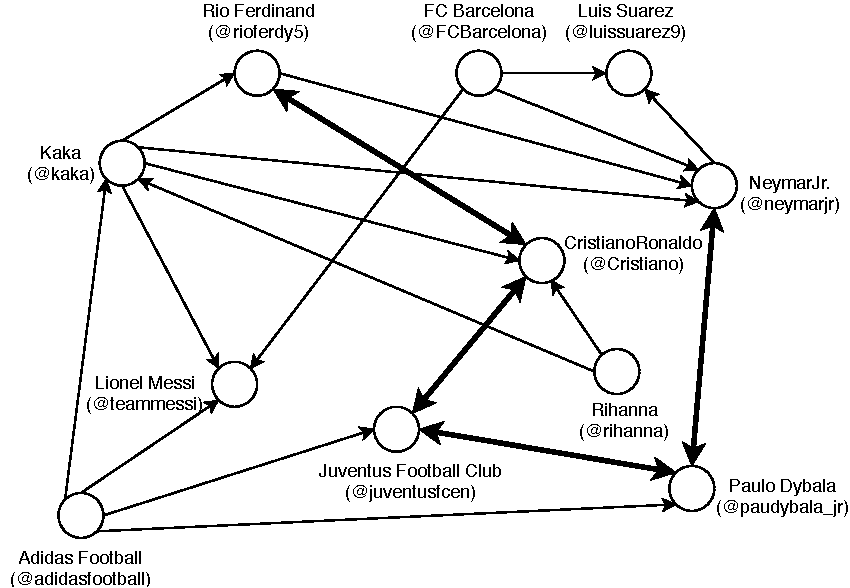
\includegraphics[width=.5\textwidth]{friend_follower_graph.pdf}
	\caption{sample Friend-Follower Graph of Twitter Social Network}
	\label{friend-follower graph}
\end{figure}

\subsection{Centrality Measurement}
In graph theory, centrality is a term to describe importance of individual vertex within a graph or a network. The concept of centrality was first developed with an intention of doing social network analysis and there has been a lot of research works carried out in this topic for network analysis mainly to answer the question, ``Which vertices are the most influential in a graph?" There are several centrality measures which are very popular in graph analysis. These measures can be categorized in two types: local and global metrics. In this section, we briefly describe various local and global centrality metrics that are available to find the influential nodes from a graph network.

\subsubsection{Local Centrality Measures}
In general, local centrality measures use only the features of an individual node through the partial information around it. The number of neighbors (degree of a node) plays the main role in such local methods and they work better mainly for undirected networks. There are mainly two local centrality measures and they are described below:

\begin{itemize}
	\item \textbf{Degree Centrality}: Degree Centrality is the simplest centrality measure which assume that the node with the maximum neighbors possess the maximum influence on the network. The degree of the node $v_i$ signifies the total number of edges incident to it i.e. the number of neighbors. Assume that, a graph $G(V,E)$ where $V$ is a set of $n$ nodes and $E$ is the edge set, is represented by an $n\times n$ adjacency matrix $A = \{a_{ij}\}$, that is $\{a_{ij}\} = 1$ if nodes $v_i$ and $v_j$ are connected and $0$ otherwise. If the degree of node $v_i$ is denoted by $d_i$, then the degree centrality of node $v_i$ is:
	
	\begin{equation}
	DC(v_i) = \dfrac{d_i}{n-1}
	\label{degree centrality eq}
	\end{equation}
	
	Here $n-1$ is the largest possible degree in $G$ and it is used as the numerator of the formula for normalization.
	
	The most important side of using degree centrality to find the most influential spreader on a network is its simplicity and low computational complexity. However, in most of the cases this measure fails to identify the most influential spreaders accurately. However, there are several use cases where degree centrality can provide surprisingly good performance such as with very small spreading rate, degree centrality is a better metric to identify the spreading influences of nodes than other well-known centrality metrics \cite{klemm2012measure,liu2016locating}.
	
	\item \textbf{K Core Decomposition}: Degree centrality only considers the number of the adjacent neighbors in order to assess the influence of a node in the network. However, Kitsak et al. \cite{kitsak2010identification} identified that the location of a node in a network has a more significant aspect in evaluating its spreading influence. Nodes located at the core of a network are more likely to have a higher influence rate than those located at the periphery. Therefore, they suggested that core value of a node is a better metric in finding most influential spreaders and the core value can be obtained by using the k-core (aka k-shell) decomposition \cite{dorogovtsev2006k} of the networks. 
	
	The $k$-shell method starts by removing all nodes having degree 1. The process is repeated until there is no node of degree 1 exists in the network. These pruned nodes are assigned into the 1-shell. After assigning the 1-shell, all nodes with residual degree 2 are recursively removed and the 2-shell are created. This procedure continues as the residual degree increases until all nodes in the nodes have been assigned to one of the shells. The nodes with high $k$-shell value tend to locate in the center of the network and the spreading starting from each of these nodes are likely to widely cover the network. In this way all nodes are assigned a \emph{k} (sometimes refereed to as $k_s$) value. Figure~\ref{fig:k core} presents a sample network and the $k_s$ value for the nodes by this algorithm. The algorithm is very simple and robust. 
	
	\begin{figure*}[htpb]
		\centering
		\subfloat[]{
			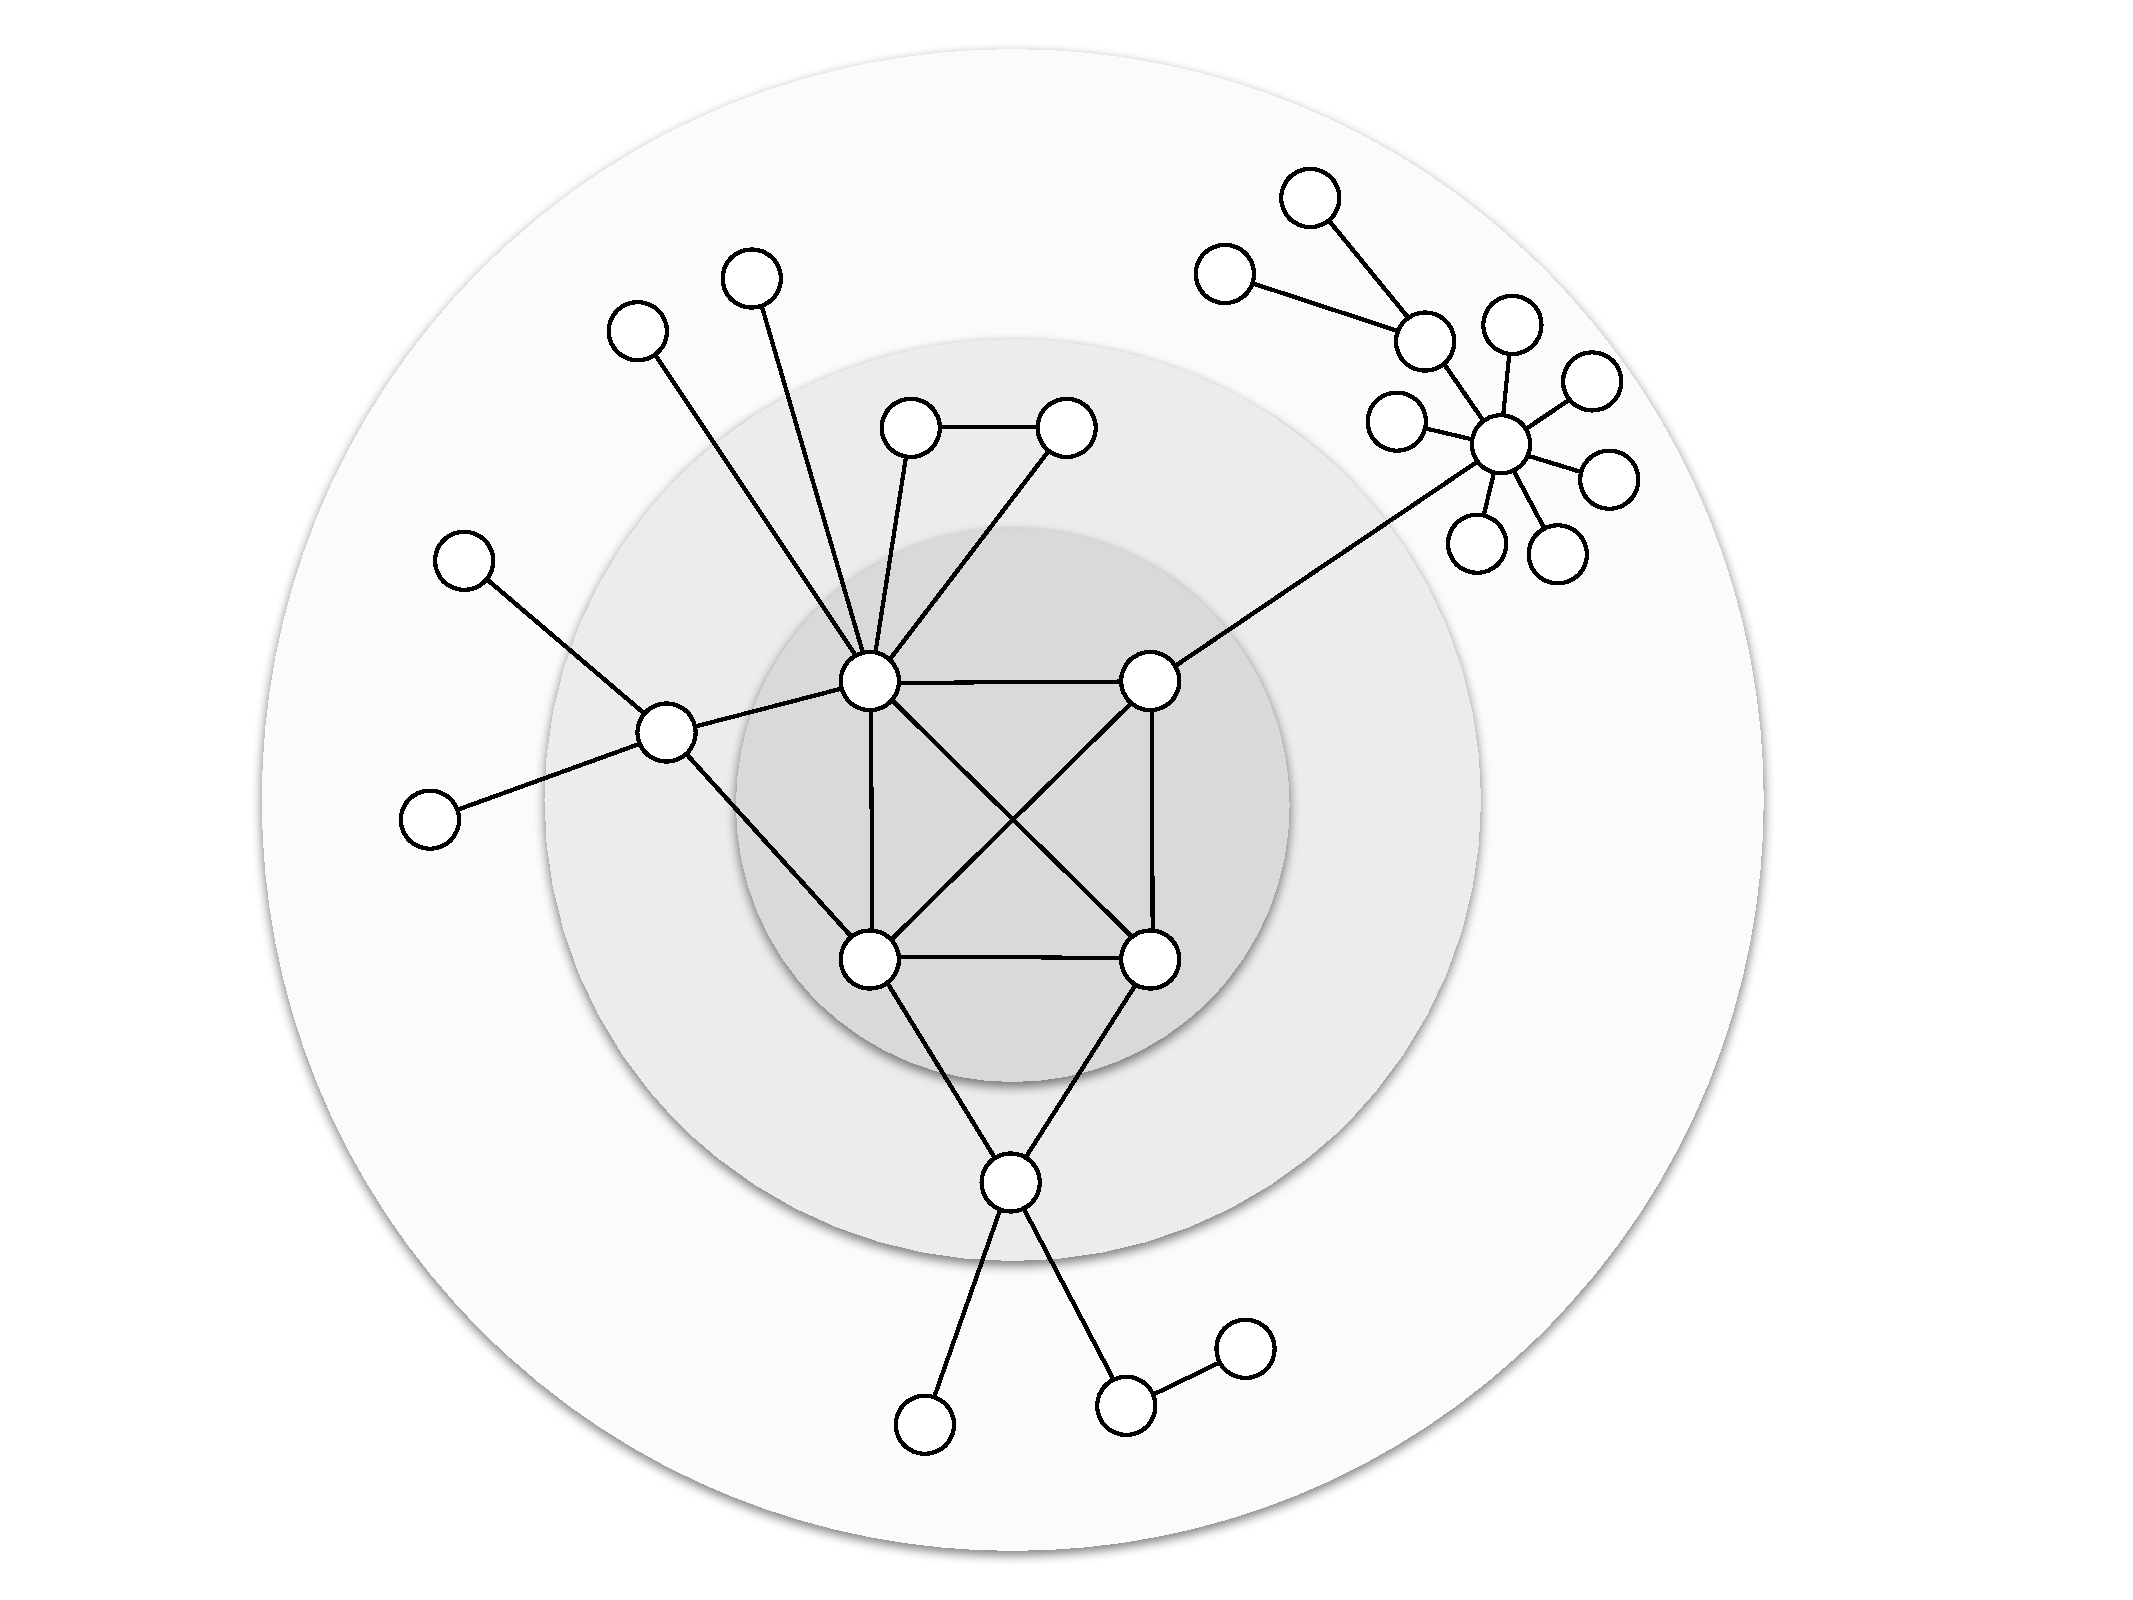
\includegraphics[width=.4\textwidth,page=1]{k_core.pdf}
			%\graphicsplaceholder{4cm}{1cm}
			\label{first-subfig}
		}
		\subfloat[]{
			%\graphicsplaceholder{4cm}{1cm}
			\includegraphics[width=.4\textwidth,page=2]{k_core.pdf}
			\label{ks=1}
		}
		\\
		\subfloat[]{
			%\graphicsplaceholder{4cm}{1cm}
			\includegraphics[width=.4\textwidth,page=3]{k_core.pdf}
			\label{ks=2}
		}
		\subfloat[]{
			%\graphicsplaceholder{4cm}{1cm}
			\includegraphics[width=.4\textwidth,page=4]{k_core.pdf}
			\label{ks=3}
		}
		\caption{A sample network with $k_s$ value of the nodes}
		\label{k core}
	\end{figure*}

	However, k core decomposition method has a tendency to assign the same $k_s$ value to multiple nodes in case of large networks. Therefore, the hypothesis of declaring the node(s) of the largest $k_s$ value i.e. the node(s) of the innermost shell to be the most influential results in a good number of nodes with the same spreadabilty and that may not be the desired outcome in many cases. However, the simplicity and lower computational complexity make this metric very useful to find the most influential nodes on a network and in this paper, we extend this idea and propose a modified k core decomposition method that can accurately find the most influential spreaders on a social network with very lower computational complexity.
\end{itemize}

\subsubsection{Global Centrality Measures}
Global centrality measures consider the whole network during its computation. There exists many different types of global centrality measures and each of them addresses slightly different properties of the network and the nodes in order to compute the centrality value. Two mostly used global centrality measures are closeness and betweenness centralities and they are described briefly below:
\begin{itemize}
	\item \textbf{Closeness Centrality}:
	As the name suggests, closeness centrality measures how close a node is from all other nodes in a network. In case of a connected graph, the normalized closeness centrality of a node is the average length of the shortest path between the node and all other nodes in the network. Let $d_{ij}$ be the length of shortest path between node $v_i$ and $v_j$, $n$ be the number of nodes of the network, then the average shortest distance of node $v_i$ will be \cite{sabidussi1966centrality},
	\begin{equation}
	Avg_i = \dfrac{1}{n-1} \sum_{i \neq j}d_{ij}
	\label{average shortest distance equation}
	\end{equation}
	Since the centrality measure is intended to find the most closer nodes, the closeness centrality of node $v_i$ is inversely proportional to the average shortest distance, $Avg_i$ and can be defined as,
	\begin{equation}
	CC(v_i) = \dfrac{n-1}{\sum_{i \neq j}d_{ij}}
	\label{closeness centrality eq}
	\end{equation} 
	
	However, this equation will not be suitable to use in case disconnected graph where some node may be unreachable from the considering node $v_i$. Wasserman and Faust \cite{opsahl2010node} proposed an improved formula for graphs with
	more than one connected component. The result is ``a ratio of the
	fraction of nodes in the network which are reachable, to the average
	distance" from the reachable nodes. Let $n_r$ be the number of reachable nodes in the network from node $v_i$, then the modified formula of measuring closeness centrality is,
	\begin{equation}
	CC(v_i) = \dfrac{n_1-1}{n-1} \dfrac{n_1-1}{\sum_{i \neq j}d_{ij}}
	\label{closeness centrality eq modified}
	\end{equation}  
	\item \textbf{Betweenness Centrality}:
	Betweenness centrality determines how many times a node falls along the shortest path between two different nodes i.e. acts as a bridge between those two nodes. 
	Linton Freeman \cite{freeman1977set} introduces this measure for quantifying the control of a human on the communication between other humans in a social network. 
	
	For starting node $v_s$ and destination node $v_t$ and the input node $v_i$ that holds the condition $v_s \neq v_t \neq v_i$, let $n_{st}^i$ be $1$ if node $v_i$ lies on the shortest path between $v_s$ and $v_t$; and $0$ otherwise. So the betweenness centrality is defined as:
	
	\begin{equation}
	BC(v_i) = \sum_{st}n_{st}^i
	\end{equation}

	However, there can be more than one shortest path between $v_s$ and $v_t$ and that will count for centrality measure more than once. Thus, if total number of shortest paths between $v_s$ and $v_t$ is $g_{st}$, the updated equation for finding betweenness centrality of node $v_i$ will be,
	
	\begin{equation}
	BC(v_i) = \sum_{st} \dfrac{n_{st}^i}{g_{st}}
	\label{betweenness centrality eq}
	\end{equation}	
	
\end{itemize} 

\subsection{Susceptible-Infected-Recovered (SIR) Model}
The SIR model is one of the simplest compartmental models in epidemiology. In an SIR model, every mode of a network can be at one of the following three states:
\begin{itemize}
	\item S (Susceptible): These denotes those people who have not been infected with the disease yet. However, they are not immune to it and therefore they are under thread of being infected with the disease in the future.
	\item I (Infected): These are people who have already been infected with the disease. Moreover, the infected people can transmit the disease to the susceptible neighbors with a probability of $\beta$.
	\item R (Recovered): These people have been recovered from the disease with a probability of $\gamma$ and are immune now. Therefore, they are no longer under any thread to be infected with the disease in future.
\end{itemize} 
The SIR model runs the simulation of disease diffusion based on the topology of the network and the probability parameters $\beta$ and $\gamma$. The simulation stops when the network has no more infected nodes. This SIR model is capable of finding the most influential spreaders based on their sreadability. 

\section{Related Work}
An online social network (\emph{OSN}) results from the use of a social network site (\emph{SNS}) that allows the users to publish messages and connect to other users which result in creating social relationships. An OSN is formally represented by a graph, where nodes are users and edges are relationships that can be either directed or undirected. In this graph the nodes play an important role to disseminate information. Finding the most influential spreader in an OSN has caught attention of the researchers. Recently more and more attentions have been paid to microscopically study the \emph{spreadability} for each node. The knowledge of node \emph{spreadability} is crucial for developing efficient methods to either decelerate spreading in the case of diseases, or speed up spreading in the case of information flow. Moreover, it can be helpful for identifying the initial spreader of certain disease or information.

Though the most connected nodes (hubs) and the nodes with high betweenness centrality are commonly believed to be the most influential spreaders in networks, the $k$-core (also called $k$-shell) method is found to perform better in identifying the best individual spreaders~\cite{kitsak2010identification,carmi2007model}. Basically, the principle of
the $k$-core decomposition is to assign a core index $k_s$ to each node such that nodes with the lowest values are located at the periphery of the network while nodes with the highest values are located in the center of the network. We shall discuss the details about the algorithm shortly. 

Cataldi et al.~\cite{cataldi2010emerging} proposed to use the well known PageRankalgorithm~\cite{page1999pagerank} to assess the distribution of influence throughout the network. The $PageRank$ value of a given node is proportional to the probability of visiting that node in a random walk of the social network, where the set of states of the random walk is the set of nodes. Both the methods only exploit the topology of the network, and ignore other important properties, such as nodes’ features and the way they process information. L\"u et al.~\cite{lu2011leaders} proposed the \emph{LeaderRank} algorithm to identify influential spreaders in directed networks, which is a simple variant of $PageRank$, namely a so-called ground node connected with every other node by a bidirectional link is introduced into the original network, and then the standard random walk process is applied to dig out influential spreaders. Li et al.~\cite{li2014identifying} further improved the $LeaderRank$ by allowing nodes with more fans get more scores from the ground node. With almost the same converging speed (we have checked by simulations), this so-called $Weighted LeaderRank$ performs better than $LeaderRank$.

Romero et al.~\cite{romero2011influence} develop a graph-based approach similar to the well known HITS algorithm, IP(i.e. \emph{Influence-Passivity}), that assigns a relative $influence$ and a $passivity$ score to every users based on the ratio at which they forward information. However, no individual can be a universal influencer, and influential members of the network tend to be influential only in one or some specific domains of knowledge. Therefore, Palet al.~\cite{pal2011identifying} developed a non-graph based, topic-sensitive method. To do so, they define a set of nodal and topical features for characterizing the network members. Using probabilistic clustering over this feature space, they rank nodes with a within-cluster ranking procedure to identify the most influential and authoritative people for a given topic. Weng et al.~\cite{weng2010twitterrank} also develop a topic-sensitive version of the $PageRank$ algorithm dedicated to Twitter, \emph{TwitterRank}. They presented the phenomenon of $homophily$ in a community of Twitter. By making use of this phenomenon, a PageRank-like algorithm, called \emph{TwitterRank}, is proposed to measure the topic-sensitive influence of the \emph{twitterers}. 

All these methods described are summarized in Table~\ref{tab:summary}. We can see that none of the above approach is distributed. Most famous approach for finding influential spreader is the $k$-core decomposition which considers only the network topology. We propose a distributed variant of the algorithm which also considers user info like no. of followers, no. of friends, whether the user is verified etc.


\begin{table}[h]
	\centering
	\caption{Summary of influential spreaders identification methods}
	\label{tab:summary}
	\begin{tabular}{|l|c|l|l|l|}
		\hline
		\multicolumn{1}{|c|}{\textbf{Algorithm}} & \textbf{\begin{tabular}[c]{@{}c@{}}Network\\ Topology\end{tabular}} & \multicolumn{1}{c|}{\textbf{\begin{tabular}[c]{@{}c@{}}User\\ Info\end{tabular}}} & \multicolumn{1}{c|}{\textbf{\begin{tabular}[c]{@{}c@{}}Topic\\ Info\end{tabular}}} & \multicolumn{1}{c|}{\textbf{Distributed}} \\ \hline
		$k$-core decomposition                     & Y                                                                   &                                                                                   &                                                                                    &                                           \\ \hline
		PageRank                                 & Y                                                                   &                                                                                   &                                                                                    &                                           \\ \hline
		Topic-sensitive PageRank                 & Y                                                                   &                                                                                   & \multicolumn{1}{c|}{Y}                                                             &                                           \\ \hline
		IP                                       & \multicolumn{1}{l|}{}                                               & \multicolumn{1}{c|}{Y}                                                            &                                                                                    &                                           \\ \hline
		Topical Authorities                      & \multicolumn{1}{l|}{}                                               & \multicolumn{1}{c|}{Y}                                                            & \multicolumn{1}{c|}{Y}                                                             &                                           \\ \hline
	\end{tabular}
	
\end{table}

\section{Our Proposed Modified K Core Decomposition Method}

\subsection{Distributed K Core Decomposition}
\label{distributed k core}
Centralized algorithms for the $k$-core decomposition already exist~\cite{batagelj2011fast}. Their algorithm is based on the recursive deletion of vertexes (and edges incident to them)
of degree less than $k$. The algorithm makes use of $bin-sort$, and can run in $O(max(m,n))$, which equals $O(m)$ for connected networks. However a distributed variant is very much needed because of two possible scenarios: the graph could be so large to not fit into a single host, due to memory restrictions; or its description could be inherently distributed over a collection of hosts, making it inconvenient to move each portion to a central site. Montresor et al.~\cite{montresor2013distributed} proposed a distributed algorithm for $k$-shell decomposition for very large graph. Their distributed algorithm is based on the property of locality of the $k$-core decomposition: due to the maximality of cores, the $coreness$ of node $u$ is the largest value $k$ such that $u$ has at least $k$ neighbors that belong to a $k$-core or a larger core. The locality property tells that the information about the $coreness$ of the neighbors of a node is sufficient to compute its own $coreness$. Based on this idea, the algorithm works as follows: each node produces an estimate of its own $coreness$ and communicates it to its neighbors; at the same time, it receives estimates from its neighbors and use them to recompute its own estimate; in the case of a change, the new value is sent to the neighbors and the process goes on until convergence.



\section{Evaluation Metrics}
\label{evaluation metrics}
In this section, we briefly present the metrics we use to evaluate the merit our proposed ranking technique against the already established ones. In the following two sections, we present the environment we use to to run our experiments, present the datasets we use to cross check the  and discuss the out 
\subsection{Modified Jaccard Similarity Coefficient}
\label{modified jaccard}
Jaccard similarity coefficient measures the similarity between two finite sets which is defined as the ratio of the intersection to the size of the union of the sample sets. Therefore, for two comparing sets $A$ and $B$, the Jaccard similarity coefficient $J(A,B)$ is,

\begin{equation}
J(A,B) = \dfrac{|A \cap B|}{|A \cup B|}
\end{equation}

In this paper, we intend to measure the similarity of top $n$ items from two different rankings. Let $a$ and $b$ are two comparing methods and $A$ and $B$ are the two generated rankings respectively, $A_n$ and $B_n$ are subsets of $A$ and $B$ respectively with top $n$ elements, then we define modified Jaccard similarity coeefiicient $J_m(A,B)@n$ as follows,

\begin{equation}
J_m(a,b)@n = \dfrac{\vert A_n \cap B_n|}{n}
\label{modified jaccard index}
\end{equation}
We use this modified metric mainly to test the proportion of the common users in the two $n$ sized sets of the most influential users obtained from the two comparing ranking algorithms. While comparing with a established method, the higher the overlap is, the more reliable the comparing ranking algorithm.


\subsection{Rank Correlation Coefficient}

In general, correlation analyses are bi-variate analyses that measure the strength of association between two variables and the direction of the relationship. In terms of the strength of relationship, the value of the correlation coefficient varies between $+1$ and $-1$. A value of $\pm 1$ indicates that there exists a perfect degree of association between the comparing two variables. As the correlation coefficient value goes towards $0$, this relationship between the two variables gets weaker. The $\pm$ sings of the coefficient indicated he direction of the relationship; a $+$ sign indicates a positive relationship while a $-$ sign indicates a negative relationship.

%In general, correlation analyses measure the strength of the relationship between two variables. They assess statistical associations based on the ranks of the data. Correlation coefficients take the values between minus one and plus one. The positive correlation signifies that the ranks of both the variables are increasing.  On the other hand, the negative correlation signifies that as the rank of one variable is increased, the rank of the other variable is decreased.

%Ranking data is carried out on the variables that are separately put in order and are numbered.

In Section \ref{?}, we measure the correlation of the ranked list of users based on their spreadability generated by our modified K core decomposition against the rankings generated by other methods. We use two non-parametric rank correlations: Kendall’s tau and Spearman’s rank correlation coefficient.

\subsubsection{Kendall Tau Correlation Coefficient}

The Kendall tau rank correlation coefficient is used to test the similarities in the ordering of data when it is ranked by quantities. While other types of correlation coefficients use the observations as the basis of the correlation, Kendall’s correlation coefficient uses pairs of observations and determines the strength of association based on the patter on concordance and discordance between the pairs. Assume that $L_1$ and $L_2$ are the two rankings that are to be compared. Then Kendall analysis takes the following two properties into consideration:

\begin{itemize}
    \item \textbf{Concordant}: Any pair of items $(x_1,y_1)$ in $L_1$ and $(x_2,y_2)$ in $L_2$ are considered as concordant if and only if they meet one of the following two conditions:
    
    \begin{itemize}
        \item ($rank\_in\_L_1(x_1) > rank\_in\_L_2(x_2)$ and 
        
        $rank\_in\_L_1(y_1) > rank\_in\_L_2(y_2)$)
        
        \item ($rank\_in\_L_2(x_2) > rank\_in\_L_1(x_1)$ and 
        
        $rank\_in\_L_2(y_2) > rank\_in\_L_1(y_1)$)
    \end{itemize}
    
    \item \textbf{Discordant}: Any pair of items $(x_1,y_1)$ in $L_1$ and $(x_2,y_2)$ in $L_2$ are considered as discordant if and only if they meet one of the following two conditions:
    
    \begin{itemize}
        \item ($rank\_in\_L_1(x_1) > rank\_in\_L_2(x_2)$ and 
        
        $rank\_in\_L_1(y_1) < rank\_in\_L_2(y_2)$)
        
        \item ($rank\_in\_L_2(x_2) > rank\_in\_L_1(x_1)$ and 
        
        $rank\_in\_L_2(y_2) < rank\_in\_L_1(y_1)$)
    \end{itemize}
\end{itemize}


 %The Kendall’s tau coefficient considers a set of joint observations from two random variables X and Y. Any pair of observation (xi, yi) and (xj, yj) are said to be concordant if the ranks for both elements agree: that is, if both xi >xj and yi >yj or if both xi <xj and yi <yj. 
 
 %They are said to be discordant if xi >xj and yi <yj or if xi <xj and yi >yj. It is defined as follows:
 
Kendall Tau correlation co-efficient is denoted by $\tau$. If $L_1$ and $L_2$ are two different rankings with $n$ similar elements, $N(C)$ and $N(D)$ represent the number of concordant and discordant pair respectively, then $\tau$ can be calculated using the following equation:
\begin{equation}
    \tau(L_1, L_2) = \dfrac{N(C)-N(D)}{\frac{1}{2}n(n-1)}
\end{equation}

\subsubsection{Spearman's Rank Correlation Co-efficient}
Spearman’s Rank correlation coefficient, $R_s$ is a technique which can be used to summarize the strength and direction (negative or positive) of a relationship between two variables.
The result will always be within 1 and minus 1. The closer $R_s$ is to $+1$ or $-1$, the stronger the likely correlation. A perfect positive correlation is $+1$ and a perfect negative correlation is $-1$. Assume that $L_1$ and $L_2$ are two rankings of same $n$ elements. For any element $x$, if the rankings of $x$ in $L_1$ and $L_2$ are $rank\_in\_L_1(x)$ and $rank\_in\_L_2(x)$ respectively, then the distance of ranks, $d = rank\_in\_L_1(x) - rank\_in\_L_2(x)$. This value is squared to remove any negative values and When written in mathematical notation the Spearman Rank formula looks like this:

\begin{equation}
R_s = 1-  \dfrac{6\sum d^2}{n^3-n}
\end{equation}
 
\subsubsection{Calculating Statistical Significance using Co-efficient Values}
Statistical significance is a measure of whether any research outcome are meaningful or not. In the field of hypothesis testing of statistics, the term \textit{null hypothesis} is the default assumption that there is no association or relationship between two measured phenomena \cite{DictionaryofStatistics}. A result has statistical significance when it is very unlikely to have occurred given the null hypothesis \cite{myers2010developing}. To be specific, a significance level, $\alpha$ is set for the experiment which denotes the probability of the experiment rejecting the null hypothesis, given that the null hypothesis were assumed to be true \cite{dalgaard2011}; and the p-value of a result, $p$ is the probability of obtaining a result at least as extreme, given that the null hypothesis were true. The result is statistically significant, by the standards of the study, when the condition $p \leq \alpha$ holds\cite{johnson2013revised,redmond2001biostatistics,cumming2013understanding,krzywinski2013points,devore2011probability}.
for the evaluation of our ranking method, we set the significance level to $5\%$.

To measure the statistical significance of the result, we use the following formula to compute a $z$-value:

\begin{equation}
z = \dfrac{3 \times T \sqrt{n(n-1)}}{\sqrt{2(2N+5)}}
\end{equation}

where $T$ is the correlation co-efficient measured by the previously described techniques. Using the $z$-score, an area is found from a z-table. This area value is considered as the $p$-value of a result.


\subsection{Normalized Discounted Cumulative Gain, $NDCG$}
In this paper, we use Normalized Discounted Cumulative Gain, $NDCG$ which is one of the widely used techniques to evaluate ranking systems. Let $GT$ represents the weighted set of all users who generate the network. The weights are the relevance of the nodes to be selected as the most influential spreader on the network and the set $GT$ is sorted according to this relevance value. We can refer to these relevance values and the ranking of the nodes in this set as our ground truth.

Now let $X$ be the ranking of nodes to be the most significant spreaders identified by any comparing method. We define cumulative gain for first $m$ rankings in $X$, $CG@m$ as:

\begin{equation}
CG@m = \sum_{i=1}^{m} rel_i
\end{equation} 
Where $rel_i$ indicated the relevance value (from ground truth) of node at rank $i$ in $X$.

Discounted cumulative gain ($DCG$) penalizes each relevance value based on its rank in the results. Therefore, we define Discounted cumulative gain for first $m$ rankings in $X$ as:

\begin{equation}
DCG@m = \sum_{i=1}^{m} \dfrac{rel_i}{log(i+1)} = \sum_{i=1}^{m} \dfrac{2^{rel_i}-1}{log(i+1)}
\end{equation}

$IDCG$ is the $DCG$ of the best possible results based on the ground truth. Therefore we define Ideal Discounted cumulative gain for first $m$ rankings in $GT$ as:
 
\begin{equation}
IDCG@m = \sum_{i=1}^{m} \dfrac{rel_i}{log(i^{(I)}+1)} = \sum_{i=1}^{m} \dfrac{2^{rel_i}-1}{log(i^{(I)}+1)}
\end{equation}

Where $i^{(I)}$ indicates the Ideal rank of a node in $GT$. $NDCG$ is obtained by dividing $DCG$ by Ideal $DCG$ ($IDCG$), which normalizes the gain within $[0,1]$. Therefore $NDCG$ for first  $m$ rankings in $X$ can be defined as,
	
\begin{equation}
NDCG@m = \frac{DCG@m}{IDCG@m}
\end{equation}

In our evaluation section we user the metric $NDCG@m(a,b)$ as the Normalized Discounted Cumulative Gain for first $m$ elements of a ranking generated by method $a$, taking the ranking generated by method $b$ as our ground truth.

\subsection{Infection Rate on SIR Model}
We use two different metrics related to infection rate on SIR model to evaluate our proposed method. These metrics were introduced by Ahajjam et al. \cite{ahajjam2018identification} and are presented below:

\subsubsection{Infection Rate Function}
This metric is used in order to compare different method of finding most influential spreaders by simulating the network on SIR model with some of the top spreaders as initially affected ones. At any time $t$, the infection rate can be defined as,
\begin{equation}
IR(t) = \dfrac{N_I(t)+N_R(t)}{n}
\label{infection rate eq}
\end{equation}
Where $IR(t)$ is infection rate at time $t$, $N_I(t)$ is number of infected nodes at time $t$, $N_R(t)$ is number of recovered nodes at time $t$ and $n$ is the total number of nodes.
 
\subsubsection{Final Infection Rate}
In order to investigate the fraction of nodes that is finally affected a metric $IR(t_{max})$ is used. When the simulation reaches a steady state, if $N_R(t_max)$ is the number of finally recovered nodes, then this metric can be defined as,
\begin{equation}
IR(t_{max}) = \dfrac{N_R(t_{max})}{n}
\label{infection rate eq}
\end{equation}





\section{Experimental Setup}
As we already have discussed, the global methods of finding most influential spreaders take large amount of time to generate the final result. Therefore, to evaluate the performance of our proposed modified K core decomposition method of finding most influential spreaders on twitter social network, we need to keep the size of the dataset considerably small. On the other hand, we run the experiments with on a distributed environment with large scaled network data which fails to run on a single computer because of memory overflow and/or take infeasible amount of time due to larger computational complexity. Consequently, we run our experiments on two different environments and they are described below:

\subsection{Cross Validation on a Single Computer}
Global metrics like closeness or betweenness centrality possess a very high computational complexity which makes them infeasible to apply on large datasets i.e. networks with large number of nodes and edges. Therefore, in order to cut off the time requirement during evaluating the performance of our proposed method against such global techniques with high complexity, we run all the comparing methods on network with smaller number of nodes and edges  
on computer with simple commodity hardware. 

\subsection{Large Network Analysis on Distributed Environment}
A number of related works for the distributed and/or parallel processing of graph structures has been presented in the literature. One popular framework for massively parallelizing
computational tasks is MapReduce~\cite{dean2008mapreduce}, introduced by Google in 2004 for the parallel processing of large data-sets. While Map-Reduce can be used for processing graphs, its structure is not optimized for such tasks. This is the reason that led Google researchers to develop another framework, called Pregel~\cite{malewicz2010pregel} which is optimized for mining graphs data~\cite{han2014experimental}. Apache Giraph~\cite{martella2012apache,martella2015practical} is the open source version of Pregel built on top of hadoop. The main idea of Giraph is ``think like a vertex''. The computation in Giraph consists of a sequence of iterations, called supersteps, during which the framework runs a user-defined function on each vertex. In this function, a node receives messages from neighbor nodes sent during the previous superstep, modifies its local state and sends messages to its neighbor nodes, to be received in the next superstep. Barrier synchronization is used, so that each superstep is separated from the next one. Individual nodes may leave the computation when they have reached the convergence to their final state.
We use Apache Giraph for implementing distributed $k$-core decomposition algorithm as described in the previous subsection \ref{distributed k core}.


\subsection{Methods Compared}
We  evaluate the merit of the ranking generated by our method against the ones generated by the following methods: 
\begin{itemize}
	\item Modified K Core Decomposition (MKC): Our method
	\item Degree Centrality (DC)
	\item Closeness Centrality (CC)
	\item Betweenness Centrality (BC)
	\item Eigenvalue Centrality (EC)
	\item HybridRank (HR)
\end{itemize}
We simulate the graph network of the datasets on the SIR model and as initially affcted nodes, we use 
the top most influential spreaders generated by all the comparing methods. We use the implementation of SIR model from the python module EoN~\cite{eon}. The input netwoks of the EoN module are NetwokX~\cite{networkx} graphs. Also we use this python module to find the centrality measures of the network. 

\subsection{Datasets Used}
In order to test the performance of our proposed modified K core decomposition method of finding most influential spreaders on twitter social network, we mainly use *** real twitter datasets. Since we compare the ranking generated by our proposed method with that of the global techniques and the global techniques take too much time to generate the results, we consider multiple subsets of the main datasets with smaller number of nodes and edges. Below we briefly describe the datasets we use for evaluating our proposed method.

\begin{itemize}
	\item We use the dataset from \cite{Kwak10www} which was collected by crawling the entire Twitter site for 6 months in 2009. This dataset contains 41.7 million of user profiles, 1.47 billion friend-follower relationships, 4,262 trending topics, and 106 million tweets. However, due to Twitter's new Terms of Services, this dataset has removed the tweet contents. Therefore, we only generate the friend-follower graph from this dataset. Since for cross validation with global techniques of finding most influential spreaders, we make two subgraphs from this dataset with smaller number of nodes and edges and we define them as follows.
	\begin{itemize}
		\item \textbf{Kwak\_50K}: We generate a subgraph from the main dataset with 50,000 randomly selected nodes and edges connecting them in the main graph. Since at every run we select a different set of randomly selected graphs, the number of average incident edges on each node vary from 1.5 to 4. We refer this dataset to \textit{Kwak\_50K} in the upcoming sections.
		\item \textbf{Kwak\_100K}: Similar to the previous one, this dataset is another subgraph generated from the main one with randomly selected 100,000 nodes and their incident edges. We refer this dataset to K\textit{wak\_100K} in the upcoming sections.
	\end{itemize}

	\item Another twitter dataset we use is collected by Kristina Lerman \cite{Lerman2010} in the year of 2010. It is a dataset containing 736,930 users and 36,743,448 links of social relationship among them. To make it feasible to run the global metrics on this dataset, we  generate a smaller dataset out of this one also with randomly selected 100,000 nodes and their incident edges and we refer to this dataset as \textit{Lerman\_100k} in our upcoming sections.
	
	\item \textbf{Twitter-Dynamic-Net}: Lou et al. \cite{lou2013learning} and Hopcroft et al. \cite{hopcroft2011will} collected this dataset for their research works. To collect this dataset, one of the known popular user on twitter was selected and then 10,000 of his/her followers were randomly collected. After that, these users were taken as seed users and a crawler was used to collect all followers of these users by traversing ``following" relationships. The total number of users is 112,044. The crawler monitored the change of the network structure among the 112,044 users during December, 2010 and finally obtained 443,399 dynamic friend-follower relationships between them. In our evaluation section, we refer to this dataset as \textit{Lou\_Hopcroft}
	
\end{itemize}

One thing to be noted that, all the smaller datasets generated from the original ones are opted to be used for cross validation of the ranking generated by our prposed mehtod. of against the established methods like 




\section{Experimental Outcome and Evaluation}

First we compare the co-efficient metrics among our comparing methods to measure their similarity in determining most influential spreaders. 
After that, we simulate the network on SIR model with some of the top most influential spreads identified by each of the comparing methods. At the end of this section, we show the $NDCG$ values of each of the rankings against the SIR geneated one and two of the mostly used methods.

\subsection{Measurement of Similarity Co-efficient among the Methods}
For establishing a ground truth, we determine the real ranking of the nodes for every dataset based on their spreadability by simulating the SIR model on the network generated from the corresponding dataset. The SIR model is simulated for 100 times with $\beta=.1$ and $\gamma=1$ and averaging the outcome, we determine the set of users ordered by their  spreadability. Using the co-efficients defined in the section \ref{evaluation metrics}, this ranking is compared with the ranked list generated by each of the comparing methods. In addition we also compare the ranked list of modified k core decomposition with each of the other methods. 


First, we measure Kendall Tau rank correlational coefficient between the ranking generated by each of the comparing methods and the one generated by SIR method. Table \ref{Kendall Tau 1} shows the results and the maximum values are shown in bold font. We can see that our proposed modified k core decomposition method mostly outperforms or give the similar better result for each of the datasets. 

modified Jaccard similarity co-efficient as defined in subsection \ref{modified jaccard}, 


\begin{table*}
	\label{Kendall Tau 1}
	\begin{adjustbox}{width={ .7\textwidth},totalheight={\textheight},keepaspectratio}%
	\begin{tabular}{|c|c|c|c|c|c|c|}
		\toprule
		Dataset &$\tau(SIR,MKC)$  &$\tau(SIR,DC)$ &$\tau(SIR,CC)$ &$\tau(SIR,BC)$ &$\tau(SIR,EC)$ &$\tau(SIR,HR)$\\
		\midrule
		Kwak\_50K & 0.87 & 0.76 & 0.78 & 0.85 & 0.71 & 0.87 \\
		\hline
		Kwak\_100K & 0.91 & 0.70 & 0.70 & 0.83 & 0.77 & 0.89 \\
		\hline
		Lerman\_100k& 0.81 & 0.71 & 0.80 & 0.82 & 0.73 & 0.82 \\
		\hline
		Lou\_Hopcoft& 0.83 & 0.73 & 0.79 & 0.81 & 0.81 & 0.82 \\
		\bottomrule
	\end{tabular}
	\end{adjustbox}
\end{table*} 

\begin{table*}
	\begin{adjustbox}{width={ .7\textwidth},totalheight={\textheight},keepaspectratio}%
		\begin{tabular}{|c|c|c|c|c|c|c|}
			\toprule
			Dataset &$\tau(MKC,SIR)$  &$\tau(MKC,DC)$ &$\tau(MKC,CC)$ &$\tau(MKC,BC)$  &$\tau(MKC,EC)$ &$\tau(MKC,HR)$\\
			\midrule
			Kwak\_50K & 0.87 & 0.76 & 0.78 & 0.85 & 0.71 & 0.87 \\
			\hline
			Kwak\_100K & 0.91 & 0.70 & 0.70 & 0.83 & 0.77 & 0.89 \\
			\hline
			Lerman\_100k& 0.81 & 0.71 & 0.80 & 0.82 & 0.73 & 0.82 \\
			\hline
			Lou\_Hopcoft& 0.83 & 0.73 & 0.79 & 0.81 & 0.81 & 0.82 \\
			\bottomrule
		\end{tabular}
	\end{adjustbox}
\end{table*} 

\begin{table*}
	\begin{adjustbox}{width={ .7\textwidth},totalheight={\textheight},keepaspectratio}%
		\begin{tabular}{|c|c|c|c|c|c|c|}
			\toprule
			Dataset &$J_m(SIR,MKC)@10$  &$J_m(SIR,DC)@10$ &$J_m(SIR,CC)@10$ &$J_m(SIR,BC)@10$ &$J_m(SIR,EC@10$ &$J_m(SIR,HR)@10$\\
			\midrule
			Kwak\_50K & 0.87 & 0.76 & 0.78 & 0.85 & 0.71 & 0.87 \\
			\hline
			Kwak\_100K & 0.91 & 0.70 & 0.70 & 0.83 & 0.77 & 0.89 \\
			\hline
			Lerman\_100k& 0.81 & 0.71 & 0.80 & 0.82 & 0.73 & 0.82 \\
			\hline
			Lou\_Hopcoft& 0.83 & 0.73 & 0.79 & 0.81 & 0.81 & 0.82 \\
			\bottomrule
		\end{tabular}
	\end{adjustbox}
\end{table*} 

\begin{table*}
	\begin{adjustbox}{width={ .8\textwidth},totalheight={\textheight},keepaspectratio}%
		\begin{tabular}{|c|c|c|c|c|c|c|}
			\toprule
			Dataset &$NDCG(SIR,MKC)@10$  &$NDCG(SIR,DC)@10$ &$NDCG(SIR,CC)@10$ &$NDCG(SIR,BC)@10$ &$NDCG(SIR,EC)@10$ &$NDCG(SIR,HR)@10$\\
			\midrule
			Kwak\_50K & 0.87 & 0.76 & 0.78 & 0.85 & 0.71 & 0.87 \\
			\hline
			Kwak\_100K & 0.91 & 0.70 & 0.70 & 0.83 & 0.77 & 0.89 \\
			\hline
			Lerman\_100k& 0.81 & 0.71 & 0.80 & 0.82 & 0.73 & 0.82 \\
			\hline
			Lou\_Hopcoft& 0.83 & 0.73 & 0.79 & 0.81 & 0.81 & 0.82 \\
			\bottomrule
		\end{tabular}
	\end{adjustbox}
\end{table*} 


\subsection{Simulation on SIR Model}
We simulate the SIR model to depict the disease diffusion based on the topology of our experimental datasets. For each method, the SIR model is simulated on the same dataset for five (5) times so that a steady result is obtained and the simulation was run for infection transition probability, $\beta = 0.1$ and recovery probability, $\gamma = 1$. We observe the simulation upto a maximum time, $t_{max} = 16$. The simulations stop when a saturation in infection spreading is achieved and Figure \ref{SIR simulation} shows the infection rate achieved with the flow of time for each of the methods on each of the datasets. Every time we select top 10 most influential spreaders identified by the comparing methods and assign them as the initially affected nodes on the SIR model. We can clearly see that the infection rate while selecting the top 10 most influential spreaders obtained by our modified k core decomposition outperforms the that of the other methods. Even though for *** , the betweenness centrality provides a better result in a very slight fraction, our method can generate  the accurate result in significantly lower computational complexity that the global methods.    


	
\begin{figure*}[!htpb]
	\centering
	\subfloat[]{
		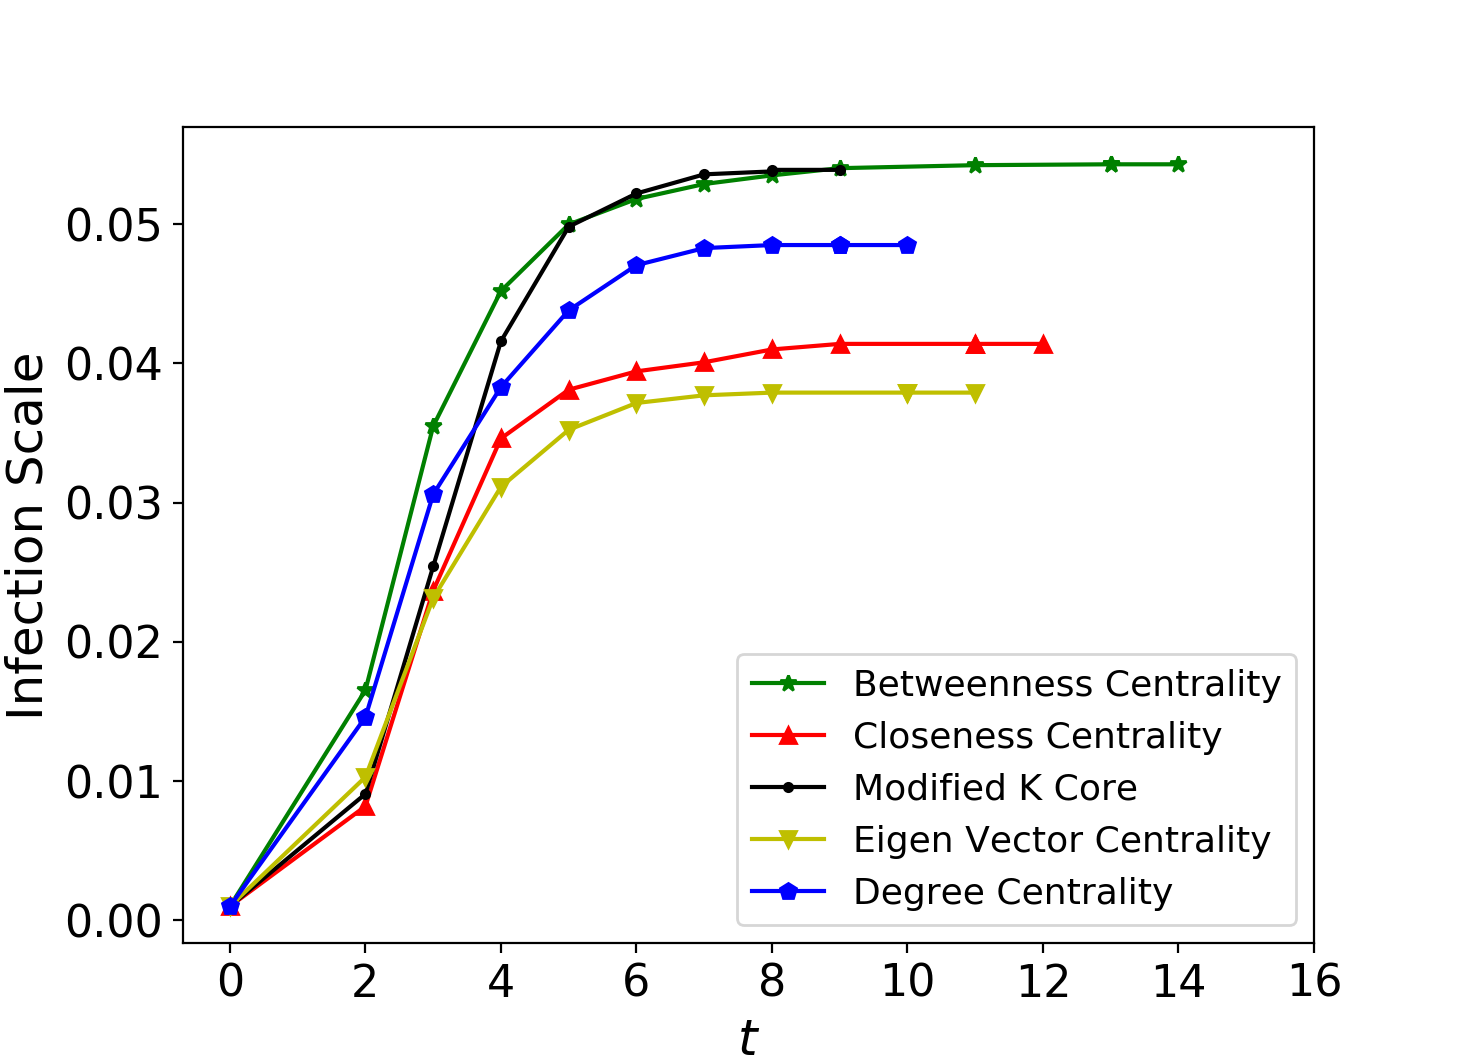
\includegraphics[width=.5\textwidth]{graphs/1.png}
		%\graphicsplaceholder{4cm}{1cm}
		\label{first-subfig}
	}
	\subfloat[]{
		%\graphicsplaceholder{4cm}{1cm}
		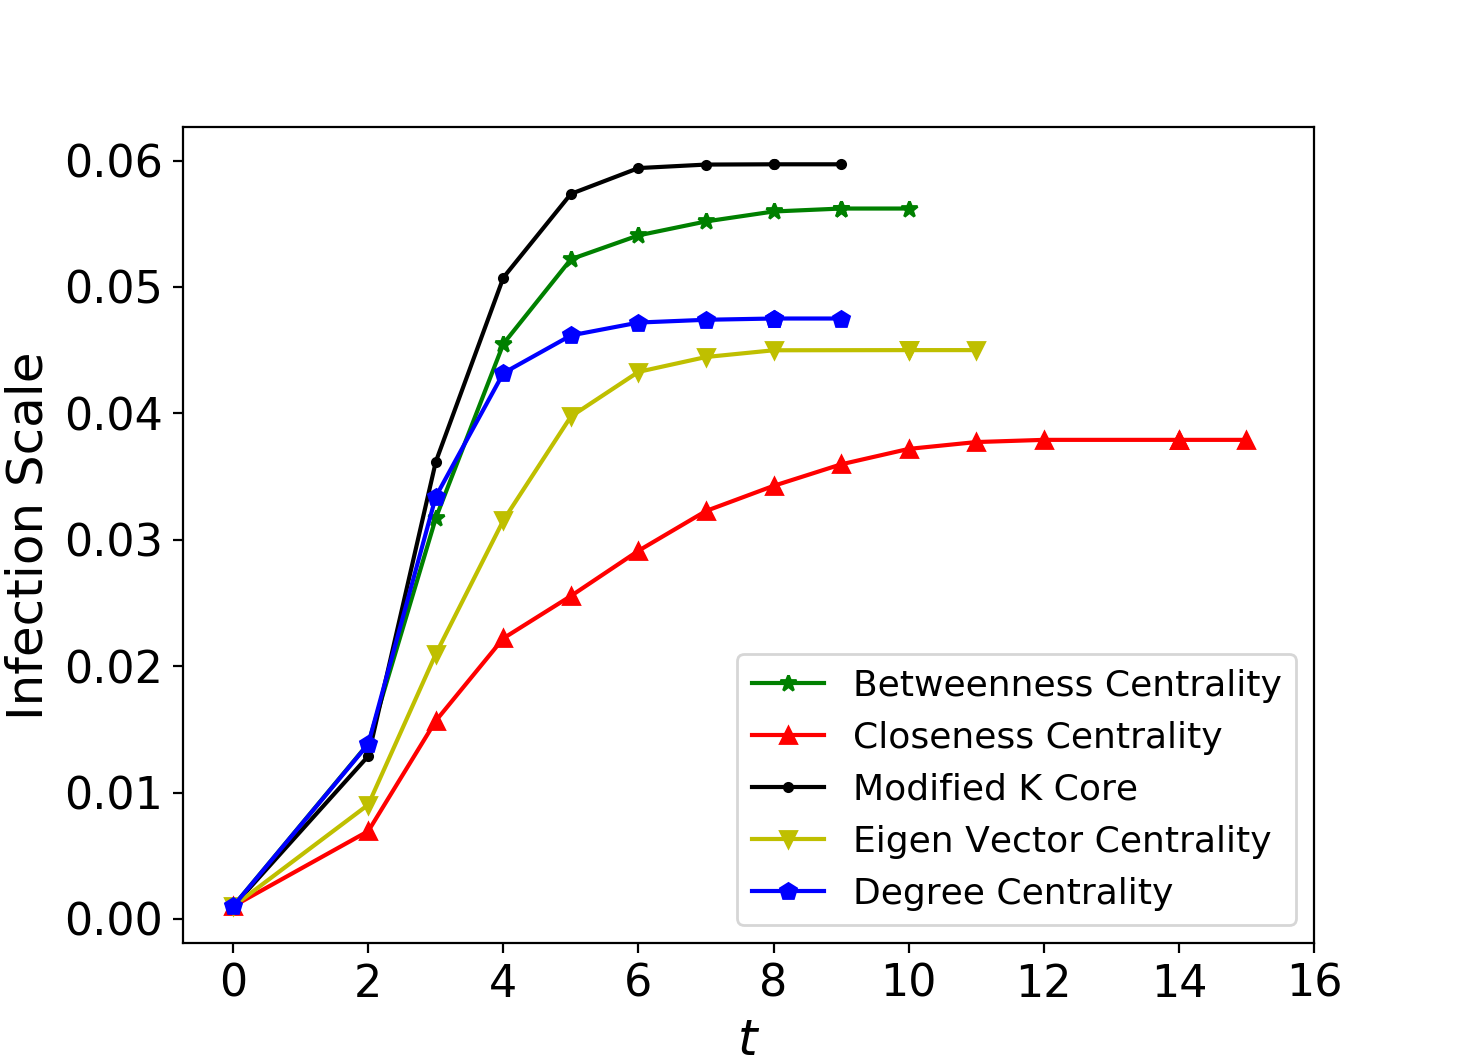
\includegraphics[width=.5\textwidth]{graphs/2.png}
		\label{ks=1}
	}
	\\
	\subfloat[]{
		%\graphicsplaceholder{4cm}{1cm}
		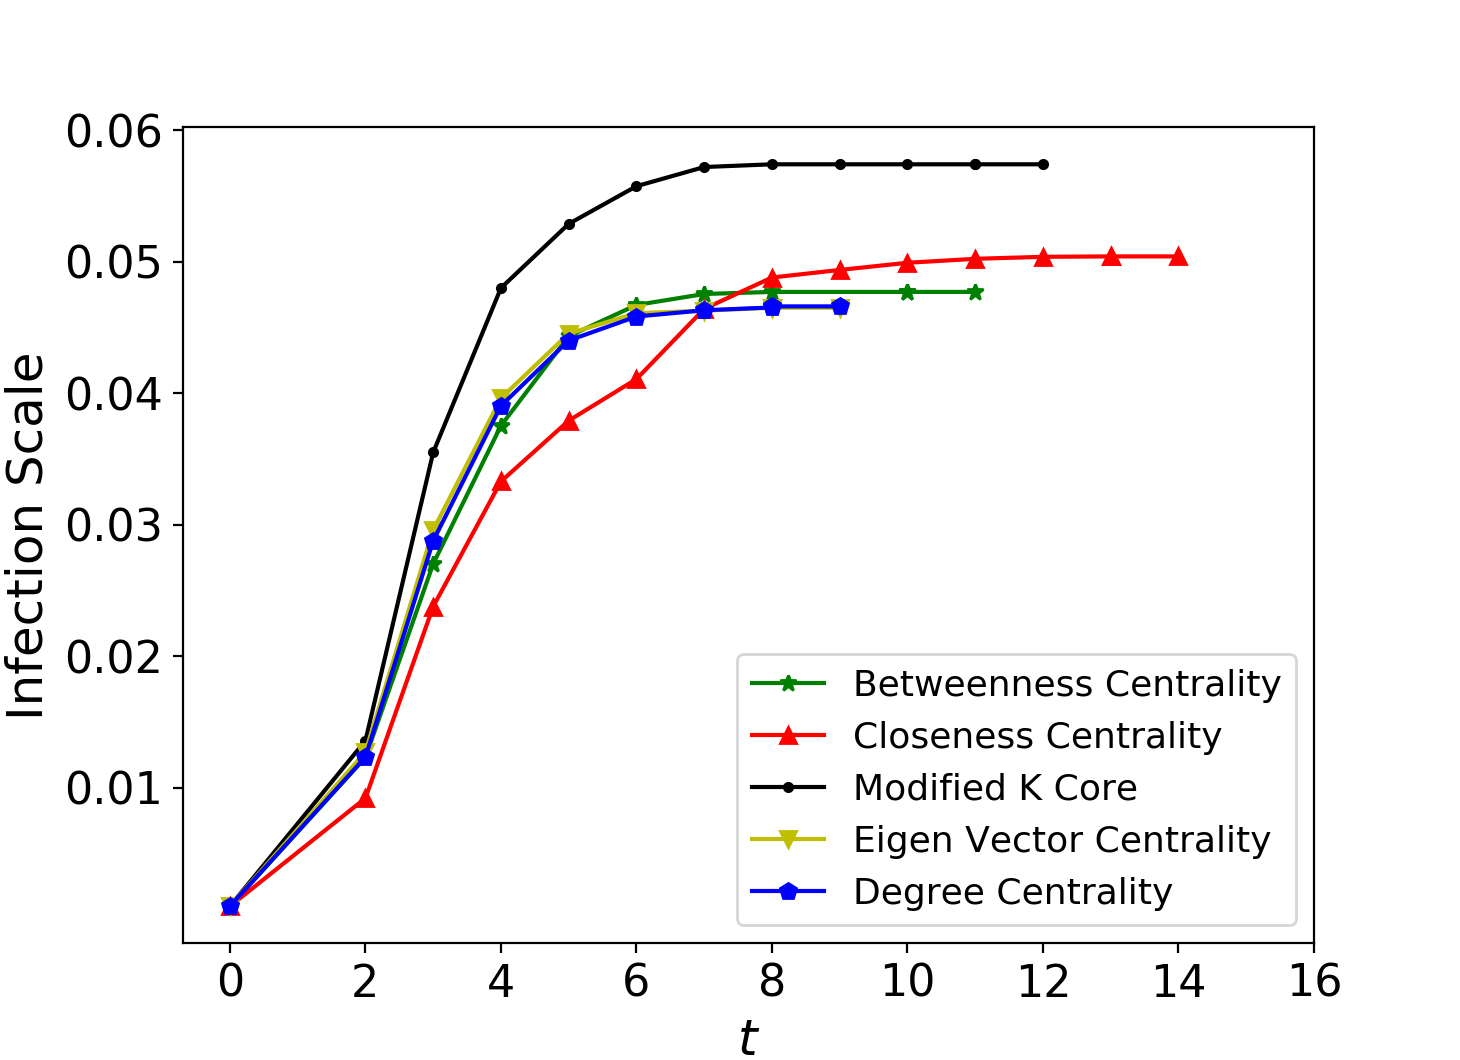
\includegraphics[width=.5\textwidth]{graphs/3.png}
		\label{ks=2}
	}
	\subfloat[]{
		%\graphicsplaceholder{4cm}{1cm}
		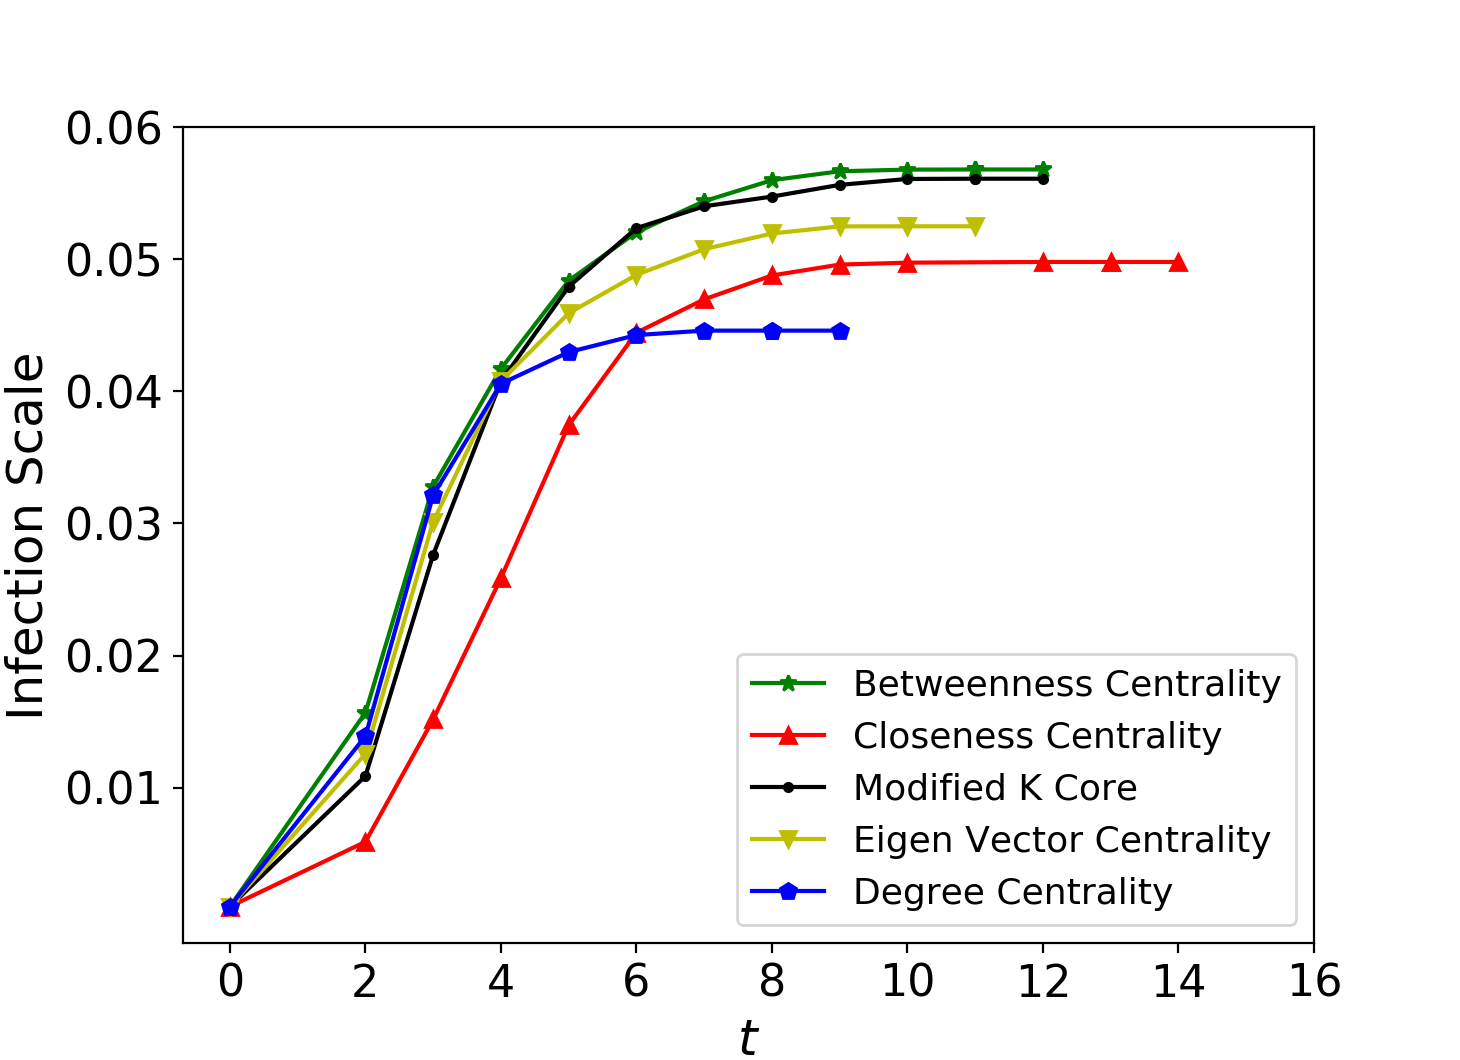
\includegraphics[width=.5\textwidth]{graphs/4.png}
		\label{ks=3}
	}
	\caption{Simulation of SIR model on 4 datasets using each of the methods.}
	\label{SIR simulation}
\end{figure*}


\section{Future Work}

\section{Acknowledgment}


\section{Conclusion}


\bibliographystyle{ACM-Reference-Format}

\bibliography{bibliography.bib}

\end{document}
